\section{Introduction}
\label{sec:introduction}

Robotic manipulation of dough and other elasto-plastic materials is difficult because every action changes both the visible geometry and the latent mechanical state. Tool contact can cause large deformation, rate-dependent response, adhesion, and irreversible shape change, while a single RGB-D camera observes only the exposed surface. These effects make broad physical data collection expensive and allow errors in reconstruction, contact, and constitutive response to produce similar image-space discrepancies \cite{sanchez2018robotic,arriola2020modeling,yin2021modeling,yazar2023doughreview,ghorbel2014adhesion}. A calibrated simulator can support controlled data generation and model-based action selection, but its predictions must first be tied to real measurements.

\begin{figure*}[t]
    \centering
    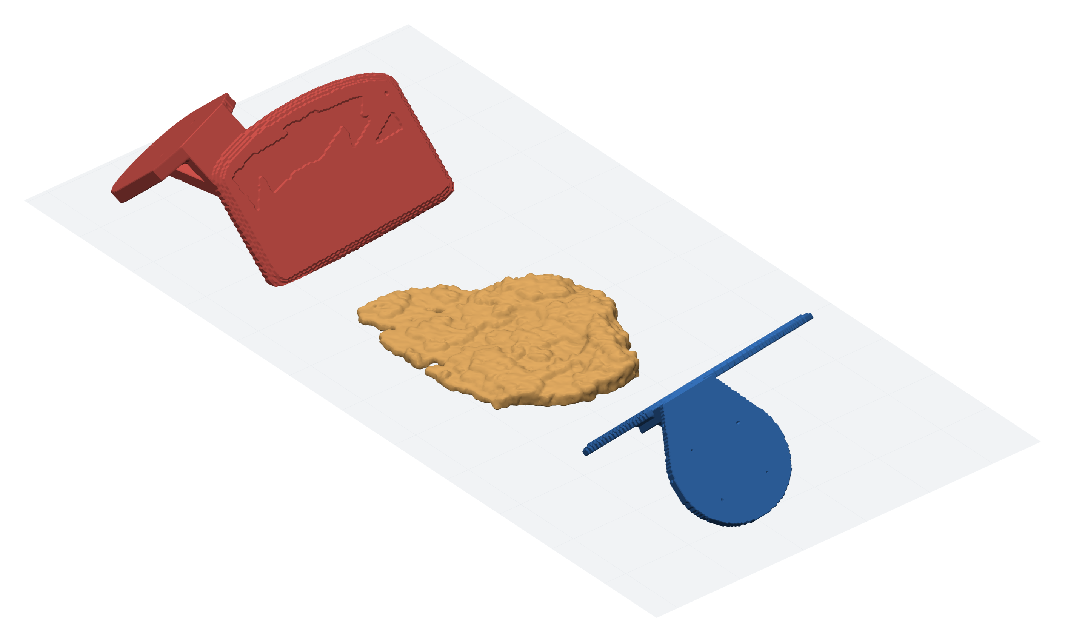
\includegraphics[width=0.60\textwidth]{figures/figure1_t0p5004.pdf}
    \caption{Simulation scene with the reconstructed dough and registered watertight signed-distance-field collision geometries of the two spatulas.}
    \label{fig:simulation}
\end{figure*}

This paper studies observation-conditioned fitting of a specified three-dimensional simulator. TaichiDough reconstructs the initially visible dough surface into a volumetric particle model, replays two motion-captured rigid spatulas in MLS-MPM, renders the resulting particles in the calibrated camera, and adjusts material-model variables to reduce disagreement with recorded depth. Figure~\ref{fig:simulation} shows the reconstructed object and registered tool geometries. The present experiment uses two spatulas, while the rigid signed-distance-field representation can accommodate other registered rigid tools; deformable end effectors would require an additional deformation model.

The fitted values are effective parameters of the declared reconstruction, contact law, constitutive model, discretization, and recorded motion rather than universal dough constants \cite{raue2011identifiability,brynjarsdottir2014discrepancy}. Robot execution and learned shaping policies are not evaluated here. The current emphasis is the calibrated sensing, replay, simulation, and fitting procedure that such downstream applications require.

The contributions are:
\begin{itemize}
    \item a metric single-view reconstruction and tool-replay pipeline combining calibrated RGB-D observations, motion-captured dual-tool motion, and mass-preserving particle initialization;
    \item a differentiable partial-view objective and bounded parameterization for fitting elastic, viscous, and principal-stretch variables in a three-dimensional MLS-MPM rollout; and
    \item an experimental analysis on one recorded sequence that quantifies objective reduction and visible-geometry improvement while documenting the resulting observation, calibration, and identifiability limitations.
\end{itemize}

\begin{figure*}[t]
    \centering
    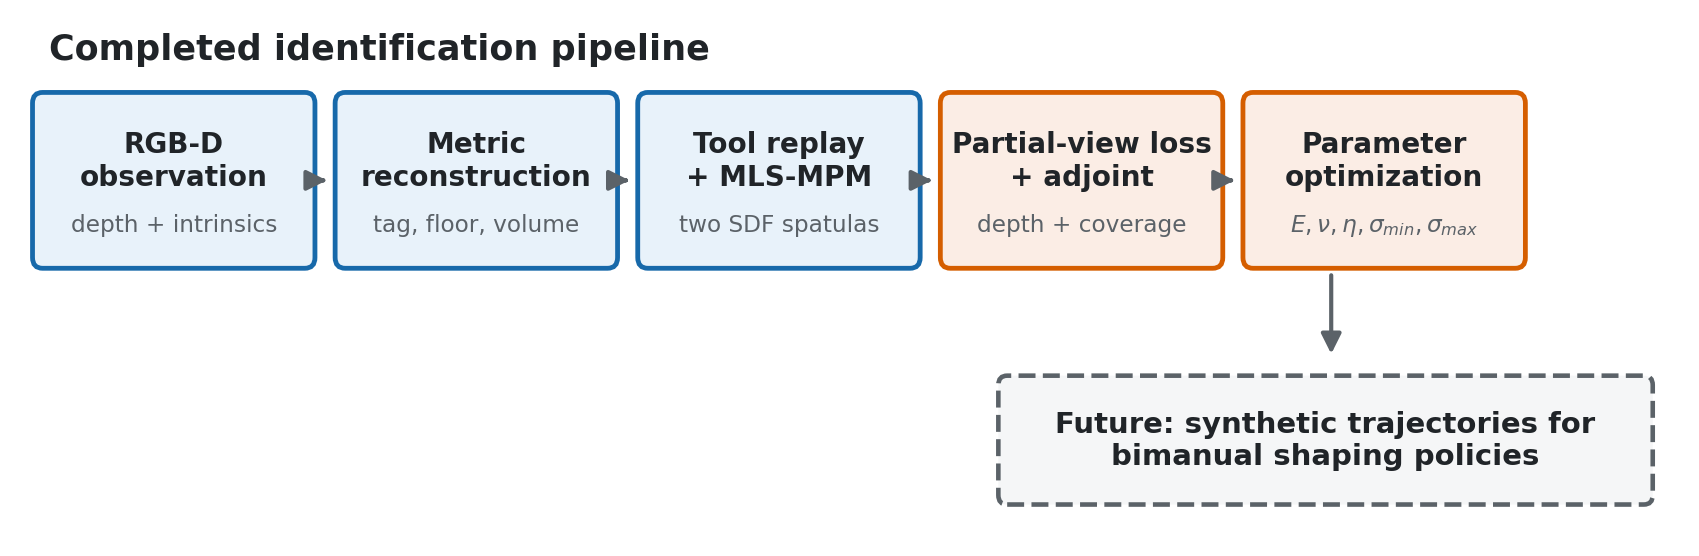
\includegraphics[width=0.98\textwidth]{figures/pipeline_overview.png}
    \caption{TaichiDough pipeline. A calibrated RGB-D camera and recorded poses of two spatulas provide the initial geometry, observations, and boundary motion. An MLS-MPM rollout is projected into the camera and compared with measured depth. Robot execution and synthetic-data learning are downstream applications rather than experiments reported here.}
    \label{fig:pipeline}
\end{figure*}

\section{Related Work}
\label{sec:related}

\textbf{Deformable object manipulation.}
Deformable object manipulation includes linear, sheet-like, and volumetric objects such as ropes, cloth, food materials, and elasto-plastic media \cite{sanchez2018robotic,arriola2020modeling,yin2021modeling}. Their state is only partially observable and evolves through contact, deformation history, and material response. Existing approaches include model-based planning \cite{jimenez2012survey}, adaptive visual servoing that estimates local motion--deformation relationships online \cite{navarroalarcon2016automatic}, and learned predictive models or policies trained from demonstrations and interaction data \cite{yin2021modeling}. G-DOOM combines learned graph dynamics with model-predictive control for rope and cloth manipulation \cite{ma2022learning}. The present work instead concerns physics-based real-to-simulation fitting for a volumetric material.

\textbf{Deformable simulation and differentiable physics.}
Simulation approaches include mass--spring systems, finite-element methods, position-based dynamics, smoothed particle hydrodynamics, and the Material Point Method (MPM) \cite{arriola2020modeling,yin2021modeling,jiang2016mpm}. MPM is well suited to large volumetric deformation because material points retain state while computation is transferred through a background grid, avoiding a permanently deforming mesh \cite{jiang2016mpm}. MLS-MPM and APIC provide the transfer formulations used here \cite{hu2018mlsmpm,jiang2015apic}. ChainQueen and DiffTaichi demonstrate gradient computation through physical simulation \cite{hu2019chainqueen,hu2020difftaichi}, while PlasticineLab applies differentiable simulation to elasto-plastic manipulation \cite{huang2021plasticinelab}. TaichiDough uses these ideas to fit a prescribed simulator against partial depth observations.

\textbf{Visual real-to-simulation fitting.}
Visual fitting methods differ primarily in observation and geometry assumptions. DiffCloud fits deformable simulations to point clouds, whereas Differentiable Depth uses a single depth camera with known reference geometry \cite{sundaresan2022diffcloud,arnavaz2023diffdepth}. PAC-NeRF jointly estimates geometry and physical parameters from multi-view video \cite{li2023pacnerf}, and PhysTwin reconstructs spring--mass digital twins from interaction videos \cite{jiang2025phystwin}. DPSI fits elasto-plastic material and contact parameters from real interactions and incomplete point clouds \cite{yang2025dpsi}, while EMPM combines multi-view RGB-D reconstruction with online MPM refinement \cite{chen2026empm}. TaichiDough examines a more restricted measurement setting: one calibrated depth view, a floor-filled initial volume, and measured dual-tool motion. This reduces sensing requirements but leaves hidden geometry, contact, and material effects mutually ambiguous.

\textbf{Robotic shaping and dough mechanics.}
RoboCraft and RoboCook learn predictive dynamics for goal-directed elasto-plastic shaping with diverse tools \cite{shi2022robocraft,shi2023robocook}, while DoughNet predicts geometric and topological changes during dough manipulation \cite{bauer2024doughnet}. Food-engineering studies instead estimate dough rheology from controlled mechanical measurements; Fabbri and Cevoli invert a finite-element model using extrusion measurements \cite{fabbri2015dough}. Dough response also depends on formulation, preparation, loading history, and adhesion \cite{yazar2023doughreview,ghorbel2014adhesion}. In contrast, the present experiment fits simulator parameters from visual motion without force measurements. Its values characterize the selected model and recorded sequence, not the complete rheology of the dough.
